\documentclass[11pt]{article}
\usepackage{tikz}
\usetikzlibrary{shapes}
\usetikzlibrary{decorations.pathreplacing}
\usepackage{amssymb}
\usetikzlibrary{arrows.meta}
\usepackage{amsmath}
\usepackage{tcolorbox}

\begin{document}

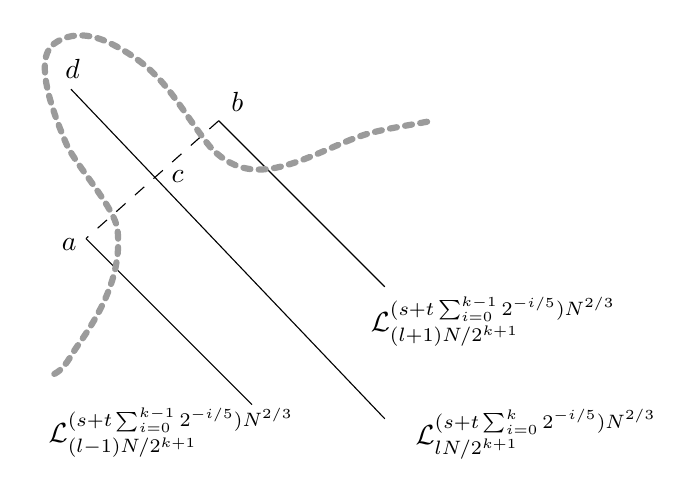
\begin{tikzpicture}[x=0.75pt,y=0.75pt,yscale=-0.8,xscale=0.8]

\draw    (240,171) -- (340,271) ;
\draw    (320,100) -- (420,200) ;
\draw    (231,81) -- (420,279.5) ;
\draw  [dash pattern={on 4.5pt off 4.5pt}]  (320,100) -- (240,171) ;
\draw  [color={rgb, 255:red, 155; green, 155; blue, 155 }  ,draw opacity=1 ][dash pattern={on 2.53pt off 3.02pt}][line width=2.25] [line join = round][line cap = round] (221,252.5) .. controls (227.57,249.22) and (230.73,241.47) .. (235,235.5) .. controls (249.53,215.15) and (262,191.49) .. (259,165.5) .. controls (257.48,152.31) and (233.05,125.77) .. (228,113.5) .. controls (222.7,100.62) and (206.81,63.63) .. (221,53.5) .. controls (231.72,45.84) and (244.4,48.2) .. (255,53.5) .. controls (285.87,68.93) and (292.79,86.86) .. (313,113.5) .. controls (317.69,119.68) and (324.63,124.9) .. (332,127.5) .. controls (356.14,136.02) and (387.32,113.87) .. (411,107.5) .. controls (422.49,104.41) and (434.33,102.83) .. (446,100.5) ;

% Text Node
\draw (224,169.4) node [anchor=north west][inner sep=0.75pt]    {$a$};
% Text Node
\draw (326,81.4) node [anchor=north west][inner sep=0.75pt]    {$b$};
% Text Node
\draw (290,128.4) node [anchor=north west][inner sep=0.75pt]    {$c$};
% Text Node
\draw (226,61.4) node [anchor=north west][inner sep=0.75pt]    {$d$};
% Text Node
\draw (216,271.4) node [anchor=north west][inner sep=0.75pt]    {$\mathcal{L}^{(s+t\sum_{i=0}^{k-1}{2^{-i/5}})N^{2/3}}_{(l-1)N/2^{k+1}}$};
% Text Node
\draw (410,204.4) node [anchor=north west][inner sep=0.75pt]    {$\mathcal{L}^{(s+t\sum_{i=0}^{k-1}{2^{-i/5}})N^{2/3}}_{(l+1)N/2^{k+1}}$};
% Text Node
\draw (437,272.4) node [anchor=north west][inner sep=0.75pt]    {$\mathcal{L}^{(s+ t\sum_{i=0}^{k}{2^{-i/5}})N^{2/3}}_{lN/2^{k+1}}$};


\end{tikzpicture}

\end{document}